\documentclass{article} % For LaTeX2e
\usepackage{nips15submit_e,times}
\usepackage{hyperref}
\usepackage{url}
\usepackage{graphicx}
\usepackage{natbib}
\usepackage{amsmath}
\usepackage{amsfonts}
%\documentstyle[nips14submit_09,times,art10]{article} % For LaTeX 2.09
\newcommand{\fix}{\marginpar{FIX}}
\newcommand{\new}{\marginpar{NEW}}

\bibliographystyle{plain}

\title{Neural Networks for Speech Recognition}


\author{
Paul Vanetti \\
\texttt{} \\
\And
Ella Kaye \\
\texttt{} \\
\And
Nathan Cunningham \\
\texttt{} \\
\And
Beniamino Hadj-Amar \\
\texttt{}
}


%\nipsfinalcopy % Uncomment for camera-ready version


\begin{document}

\maketitle


\begin{abstract}
Given audio recordings of ten people reading the digits 0 to 9, we trained a neural network on the \texttt{.wav} files and classify the digit being spoken. Following previous research we  converted the audio files into mel-frequency spectral coefficients, producing an image that can be inputted into a 2D convolutional neural network (CNN). We also compare this CNN with a recurrent neural network (RNN).
\end{abstract}


\documentclass{article} % For LaTeX2e
\usepackage{nips15submit_e,times}
\usepackage{hyperref}
\usepackage{url}
\usepackage{graphicx}
%\usepackage[natbibapa]{apacite}
\usepackage{natbib}

\bibliographystyle{plain}
%\documentstyle[nips14submit_09,times,art10]{article} % For LaTeX 2.09



\begin{document}

\section{Introduction}
Given audio recordings of ten people reading the digits 0 to 9, we wish to train a computer to take the \texttt{.wav} files and accurately classify the digit being spoken. We follow \cite{abdel2014convolutional} by converting the audio files into mel-frequency spectral coefficients, producing an image that can be inputted into a 2D convolutional neural network (CNN). We also compare this CNN with a recurrent neural network (RNN). 
\bibliography{digits_bib}

\end{document}


\documentclass{article} % For LaTeX2e
\usepackage{nips15submit_e,times}
\usepackage{hyperref}
\usepackage{url}
%\documentstyle[nips14submit_09,times,art10]{article} % For LaTeX 2.09
\newcommand{\fix}{\marginpar{FIX}}
\newcommand{\new}{\marginpar{NEW}}

%\nipsfinalcopy % Uncomment for camera-ready version

\begin{document}


\section{Data}
We fit our model to a subset of the TIDIGITS dataset. The data, collected by Texas Instruments, contains audio files of over 300 speakers reciting the digits "zero" (and "oh") through to "nine" a number of times and in a variety of combinations. The dataset includes men, women, and children speaking in a number of dialects. Our subset includes just ten speakers, five men and five women, who repeat each of digit, in isolation, just twice. While the data were originally recorded at 20kHz, our subset is at 8kHz.
We split the data into a training set (consisting of three male and three female speakers) and a test set (two male and two female). In all, we trained our model on 132 samples and assessed our results on 88 samples.

 

\subsection{Data preprocessing}
After reading the data as wav files into Python, we processed them prior to analysis. 

\begin{itemize}
\item \textbf{Normalising} We normalised each of the $.wav$ files to mean 0, standard deviation 1.

\item \textbf{Cropping and padding} As the data were not uniformly padded with silence, we cropped each recording to remove silence at both ends of the audio file. In order to ensure our classifier was invariant to shifts along the time-axis we padded the beginning and end of each sample with silence of varying lengths. 

\item \textbf{Mel-frequency cepstral coefficients}
The Mel-frequency cepstral coefficients (MFCC) representation of a sound is often used in speech recognition.\cite{abdel2014convolutional} The MFCC aims to more-closely approximate the human auditory system as the frequency bands are equally spaced on the mel scale. 

We derived the MFCC as follows:
\begin{itemize}
\item Take the Fourier transform across a Tukey window of the signal
\item Take the log of these powers
\item Convert these onto the mel scale using Tukey windows
\item Take discrete cos of list of mel log powers
\item MFCC
\end{itemize}
\item \textbf{•}

\end{itemize}



\end{document}




\section{Convolutional Neural Networks}
\label{sec:cnn}
A Convolutional Neural Network (CNN) is a particular type of Artificial Neural Network (ANN). Similarly to an ANN, it receives an input and returns an output, through a series of hidden layers. Furthermore, it learns its parameters by minimising an error function, usually by performing backpropagation. 

As opposed to an ANN, where each input is typically fully connected with neurons of the next layer, a CNN instead has sparse connectivity. Each neuron in the hidden layer is connected only to a local part of the input and output. In a high-dimensional scenario full connectivity would yield an extremely large number of parameters, leading to overfitting.

Often, CNNs make the assumption that the inputs are images, constraining the architecture of the layers in 3 dimensions: \textit{width}, \textit{height}, \textit{depth}. An illustration of the structure is given below:

\begin{figure}[htbp]
	\centering
	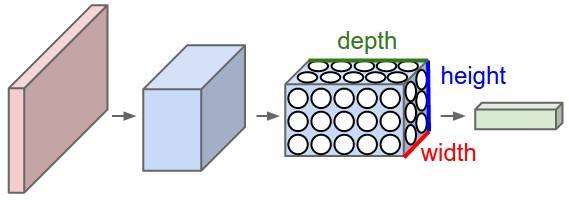
\includegraphics[scale=0.5]{cnn.png}
	\caption{The architecture of a CNN, where each layer is organised in three dimensions. Notice that each layer transforms a 3D input to a 3D output. Graphic sourced from \cite{CS231n}.}
	\label{CNN}
\end{figure}
\vspace{0.3cm}
A CNN is represented as a list of layers, where each layer transforms an input volume to an output volume through a differentiable function. There are distinct type of layers and activation functions; a typical structure could contain:
\begin{itemize}
	\item \textbf{Input} - a representation of the input image, for example a [128x128x3] volume for an image of width 128, height 128 and 3 channels for the colors RGB. 
	\item \textbf{Convolution} - an operation convolving a set of weights with the input volume; this is done by performing dot products between local regions and the weights. As a result we obtain another volume, for example of size [128x128x12]. The depth parameter is analogous to the number of hidden layers in ANN, and it controls the number of neurons in the convolution layer that connect the same local region of the input volume. 
	\item \textbf{ReLU} - a function that performs elementwise activation of the component of the volume, specifically $\max(0, x)$. Notice that in this stage the dimension of the volume is unchanged. 
	\item \textbf{Max Pooling} - a layer that reduces the dimension of the image (width and height), by selecting the maximum entry of a given region. This effectively downsamples the volume in the spatial dimensions.
	\item \textbf{Fully connected} - a layer in which each neuron is connected to all neurons of the previous layer as in an ANN, without weight-sharing or sparsity.
\end{itemize}

In this way, a CNN converts the original input image to the final category score, layer by layer. In the same way as an ANN, the parameters of the network can be trained with gradient descent.

Building an efficient CNN involves choosing the configuration of layers. Firstly, the \textit{depth} of convolution layers must be chosen; controlling the number of neurons that connect to the same region of the input volume. 
Secondly, we need to fix the \textit{receptive field}, which is the size of the local region of the input that we will convolve. Thirdly, we have to specify the \textit{stride} with which the receptive field will look at the input image; the bigger the stride, the smaller the output volume. Finally,  it is sometimes necessary to pad the input volume with zeros along the borders; so we also need to specify this parameter, called \textit{padding} that allow us to control the spatial size of the output volume. 



% We follow the model of \cite{abdel2014convolutional} wherein we first extract a two-dimensional spectrogram-like representation of the speech. We then apply a convolutional neural network to map this representation to a label. The representation used is simply a spectrogram which has been projected onto a log-frequency basis.

A spectrogram is a two dimensional representation of an audio waveform, often used to visualize speech and music. It expresses time in the horizontal axis and frequency in the vertical axis. Figure~\ref{fig:waveform} and \ref{fig:spectrogram} shows an example of this correspondence. In the example of Figure~\ref{fig:waveform} and in our experiments, the audio is sampled at 8kHz, and the frames of the spectrogram cover 256 samples (32ms) beginning every 32 samples (4ms).

Using the spectrogram we can read how the frequencies of the audio change over time. Each column of pixels in the spectrogram is the discrete Fourier transform of a ``frame'' - a short contiguous time slice of the waveform. These frames are equally spaced and of equal length, and are ordered by increasing time. The frames can overlap to create a smoother spectrogram. Each row of pixels in the spectrogram represents a frequency: the lowest row represents the constant component; the top row represents 4000 Hz (half the sampling frequency). The rows between are spaced linearly in the frequency space. The light-coloured bands we see in the spectrogram are the regions of high energy - these bands give some sense of the quality of the audio tone, and of its pitch.

The linear spacing of the frequency representation is not representative of human auditory perception, as humans hear multiplicative differencies in frequency as equivalent throughout the auditory range. As such, a shift in pitch - without a change in any other quality of the sound - would create a linear shift in the log-frequency domain, but a more complicated transformation in the spectrogram.

As such, we transform the spectrogram by mapping each column onto a log-frequency basis. These bases are spaced evenly in the mel scale; a mel is equivalent to $c \log(1 + f / 700)$ where $c$ is some constant and $f$ is the frequency in Hz. See Figure~\ref{fig:mfsc}, which is the mel-frequency transformation of the spectrogram in Figure~\ref{fig:spectrogram}.


\begin{figure}
\centering
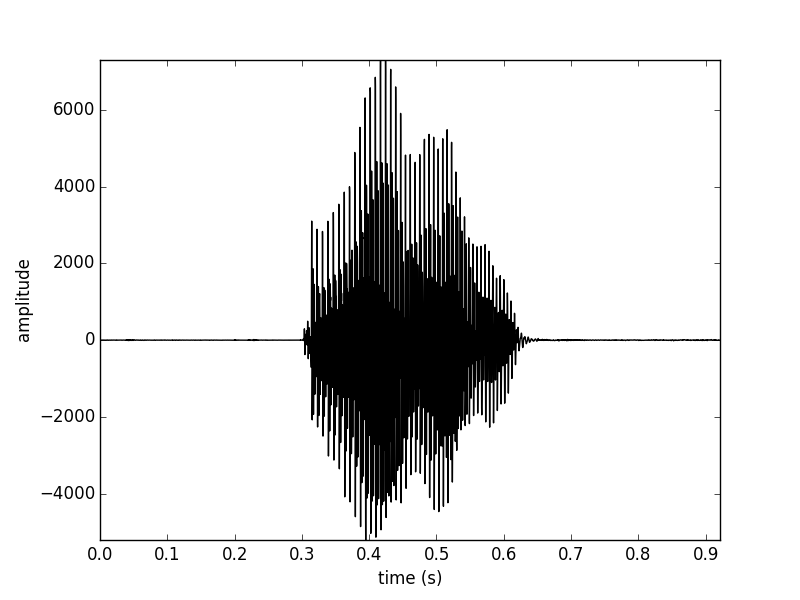
\includegraphics[width=0.8\textwidth]{waveform.png}
\caption{Waveform of the spoken word ``zero''. Cropped from the original and padded to a set length.}
\label{fig:waveform}
\end{figure}


\begin{figure}
\centering
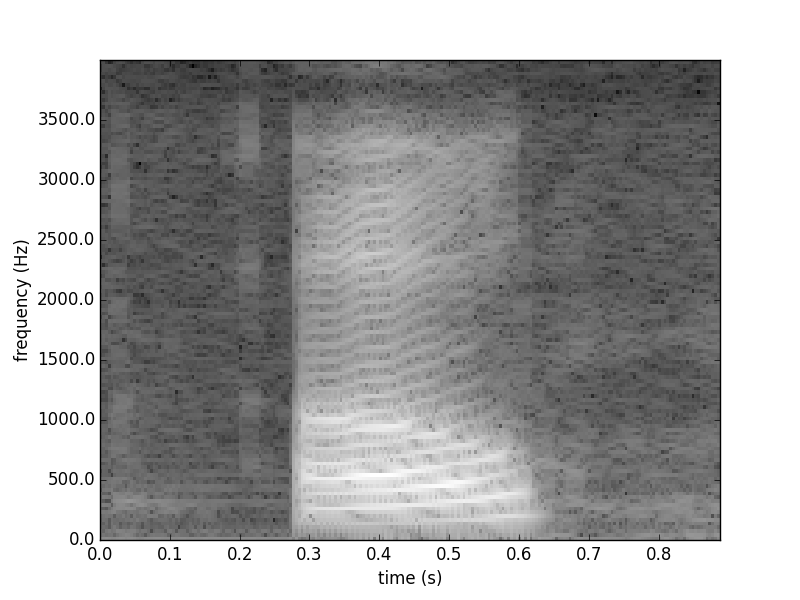
\includegraphics[width=0.8\textwidth]{spectrogram.png}
\caption{Spectrogram corresponding to the waveform in Figure~\ref{fig:waveform}.}
\label{fig:spectrogram}
\end{figure}



%\begin{figure}
%\centering
%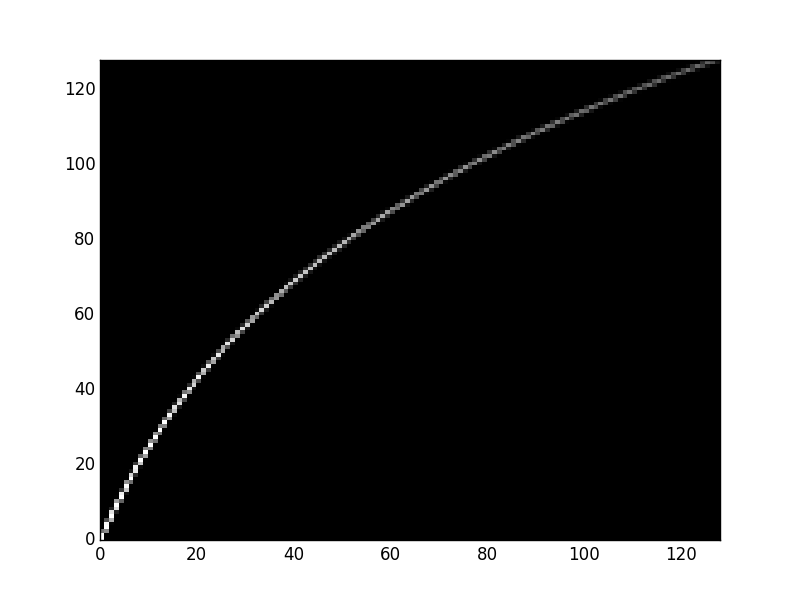
\includegraphics[width=0.8\textwidth]{mel_basis.png}
%\caption{}
%\label{fig:mel_basis}
%\end{figure}


\begin{figure}
\centering
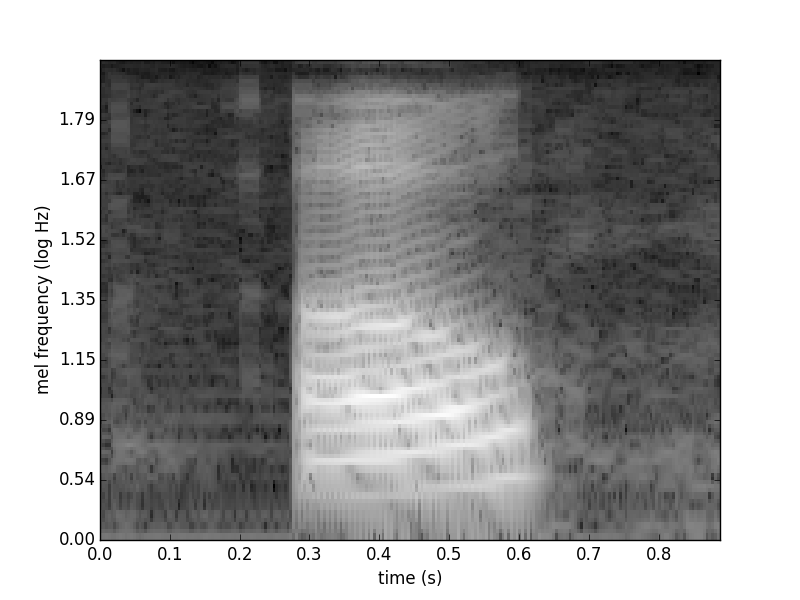
\includegraphics[width=0.8\textwidth]{mfsc.png}
\caption{Mel-frequency basis representation of the spectrogram in Figure~\ref{fig:spectrogram}. The high energy bands in the lower frequencies are spread further apart, while the high frequency bands are now closer.}
\label{fig:mfsc}
\end{figure}

















\documentclass{article} % For LaTeX2e
\usepackage{nips15submit_e,times}
\usepackage{hyperref}
\usepackage{url}
\usepackage{graphicx}
%\documentstyle[nips14submit_09,times,art10]{article} % For LaTeX 2.09



\begin{document}

\section{Models}
\subsection{Convolution Neural Network}
Our CNN model consists of eleven layers: two 2D convolution layers followed by a max pooling layer, then three alternating 2D convolution layers and max pooling layer pairs, then two dense layers at the end. In each layer, we used rectified linear units as the activation (ReLU), with the exception of the final categorisation layer, for which we used a softmax activation. 
 
\subsection{Recurrent Neural Network}

\section{Results}
\subsection{Convolution Neural Network}
We split our data into training and test sets, using six speakers for training (three male, three female) and four speakers for the test set (two male, two female). This lead to 132 samples in the training set and 88 samples in the test set. We trained the CNN using a batch size of four. For our loss function, we minimised the categorical-crossentropy.

We began by using the state-of-the-art adadelta optimiser, for training for twelve epochs. For our first runs, we did not augment the data set. We ran the network six times and obtained a wide range of results for the test accuracy. Five of the six results were in the range 0.8750-0.9432, the other was 0.0909 which, with eleven categories, is equivalent to random guessing. The validation and test accuracy for one run, as the number of epochs increases, is shown in Figure \ref{fig:2d_acc}. It appears that we are overfitting to the training data, given that the validation accuracy goes to 1. 

\begin{figure}[h]
\begin{center}
%\framebox[4.0in]{$\;$}
%\fbox{\rule[-.5cm]{0cm}{4cm} 
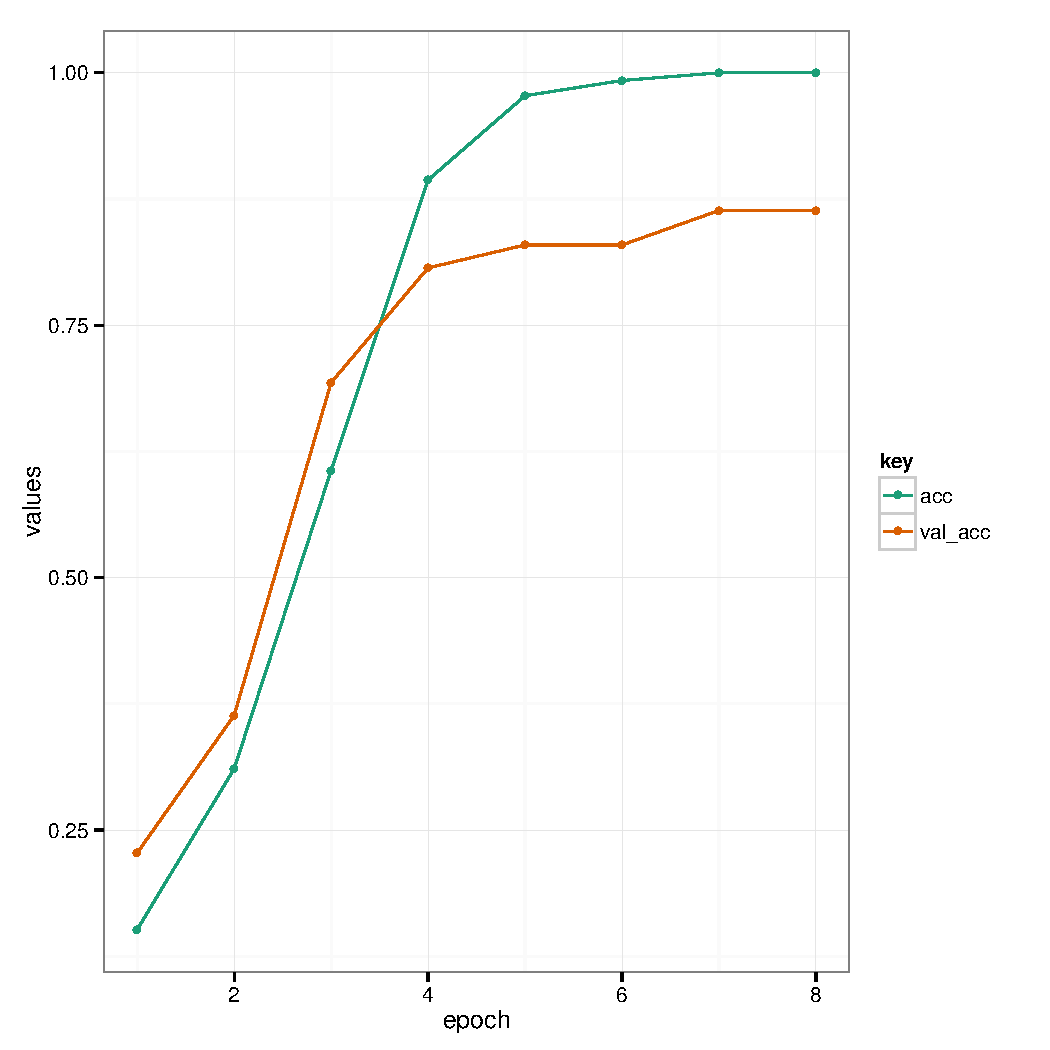
\includegraphics[height = 4in, width = 4in]{cnn_2d_plot_acc.pdf}
%\rule[-.5cm]{4cm}{0cm}}
\end{center}
\caption{Validation (red) and test (green) accuracy for the CNN on one run, with unaugmented data.}
\label{fig:2d_acc}
\end{figure}

We then ran the model with leave-one-out cross-validation (LOOCV), training on nine of the speakers and testing on the tenth. Three times out of 10, the test accuracy was 1, twice it was 0.8636 and the other half of the times it was just 0.0909.

We experimented with adding dropout layers to the CNN in an attempt to address overfitting, but did not see any improvements in the test accuracy as a result. In an attempt to improve performance, we augmented the data by copying and shifting the signal of the audio files of the training data before computing the mfsc. We shifted each training sample by each of two, four, six, eight and ten 8000th of a second to both the left and right, resulting in eleven very slightly varying training samples for every one in the original runs. This increase in the training set meant that fewer epochs were required for convergence, with results stabilising after around five. When using the original training/test data spilt, it also lead to some higher test score accuracy than in the un-augmented case, though there was still a range of results, from 0.8750-0.9659, with occasional results of 0.0909. It is not clear whether the augmentation of the data led to an improved classifier or whether the higher scores are down to some of the randomness inherent in the process.
LOOCV on the augmented training set faced similar issues as on the original set; whilst five scored highly, the other five were essentially guesses.

We also explored augmenting the original dataset by adding some white noise to the background of the audio signal, but this did not make any appreciable difference to the test scores, likely because the original audio files were all recorded in controlled settings, so there was no noise in the test set.

Since our classifer was on occasion producing very high losses, we explored the possibility that this might be because the learning rate was too high, and so ran our model again with the but optimising with stochastic gradient descent (SGD), rather than adadelta, and running for 20 rather 12 epochs. Applying LOOCV on the un-augmented training set resulted in a test accuracy of 0.8636. As with LOOCV using adadelta, the test accuracy varied greatly in each fold, ranging from 0.4545 to 1, though unlike the previous case, even its worse performance was a significant improvement on random guessing. An area of further research would be to experiment with the tuning parameters of SGD (learning rate, momentum and decay) to see if we can reduce the range and improve the average test accuracy. It would also be interesting to examine the audio files and mfsc representation of the test samples in the folds where the test accuracy was low to determine whether there is anything in particular about those speakers which makes their spoken digits harder to classify. 


\end{document}


\bibliography{digits_bib}

\end{document}
